\chapter{Umsetzung}
\todo{\dots}

\section{DataBean und DataProxy}
\todo{citeing} \citep{gamma_entwurfsmuster:_2009}
Input und Output der einzelnen Pipelinefilter ist ein einziges
Datenobjekt vom Typ \code{DataBean}. 
\index{DataBean}
\index{Klasse!DataBean}
\name{DataBean} ist nach dem Konzept der \name{JavaBeans}
\footnote{\todo{JavaBean wasdas?}}
entworfen und ist mit hierfür typischen Funkionalitäten wie Serialisierung und
öffentlicher getter und setter Methoden ausgestattet.
\index{JavaBean}
\name{DataBean} bietet den Steps der Pipeline die Möglichkeit, ihre
(Zwischen-)Ergebnisse zentral abzuspeichern.
Die zu annotierende Inputsequenz \todo{name?} ist dabei ebenfalls Teilmenge der
von \name{DataBean} gespeicherten Daten.

Da es nur ein einziges Objekt vom Typ \code{DataBean} geben soll, das zentral
und für jeden Step innerhalb der Pipeline verfügbar ist, wird der Zugriff auf
dieses Objekt an einen Proxy
\footnote{\todo{proxy pattern? \citep{freeman_entwursmuster_2005}}}
delegiert.
Dieser übernimmt zudem die Implementierung einer geeigneten
Serialisierungsstrategie und synchronisiert die Zugriffe auf das
dahinterliegende \todo{doofes wort} \name{DataBean}.
Durch den Proxy ist die kongrekte Implementierung der Datenhaltung
\todo{anderes Wort ?!} vom Rest der Pipeline getrennt und kann leicht verändert
werden.
So wäre es beispielsweise denkbar, die Daten nicht local in einem Java Objekt
abzuspeichern, sondern entfernt in einer Datenbank abzulegen. \todo{toller
satz -.-}

Der \name{DataProxy} ist innerhalb der Pipeline ein \name{Singleton}
\footnote{\todo{singleton pattern wasdas}}.
Eine Referenz auf \name{DataProxy} ist Input für jeden Step und enthält nach
dessen Ausführung auch den Output.
Der Zugriff durch die Steps soll daher per \name{call by reference} erfolgen.

\begin{figure}[htbp]
	\begin{center}
		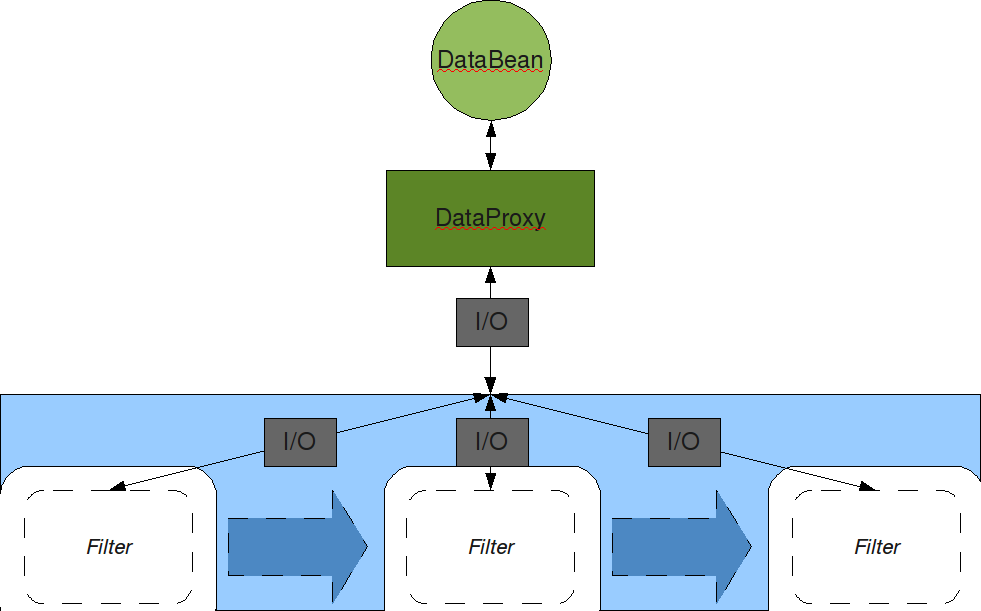
\includegraphics[scale=0.55]{pics/pipesFilter41.png}
	\caption[pipesFilter41]{
	\textbf{pipesFilter41.}
	something.}
	\end{center}
	\label{fig:pipesFilter41}
\end{figure}

\begin{figure}[htbp]
	\begin{center}
		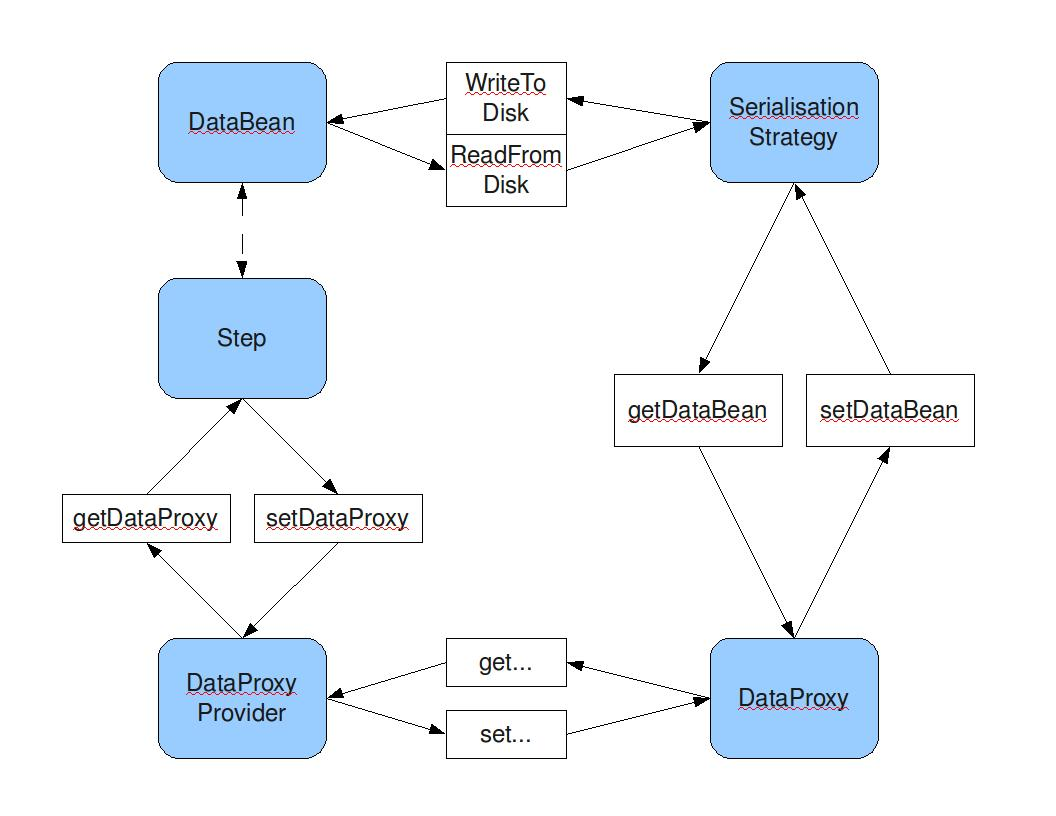
\includegraphics[scale=0.42]{pics/programDataManagment.jpg}
	\caption[Data Management]{
	\textbf{Data Management.}
	something}
	\end{center}
	\label{fig:programDataManagment}
\end{figure}
\section{Step und AbstractStep}
Ein \name{Step} implementiert das gleichnaminge Interface, das drei
Call-Back-Methoden bereitstellt, die nach der Anmeldung am Server durch diesen
ausgeführt werden.
\index{Interface!Step}
Als Parameter erhalten diese Methoden jeweils eine Instanz auf den
pipelinezentralen \first{DataProxy} \seec{chp:data}.
\index{DataProxy}
\index{DataBean}

\lstinputlisting[frame=single,label=step,caption=Das Step Interface]{code/step}

\code{AbstractStep} stellt einen abstrakten Prototyp für eine Implementierung
von \code{Step} bereit.
\index{Klasse!AbstractStep}
Diese Klasse enthält bereits wiederkehrende Funktionalitäten wie das
Anmelden am Server, das Bereitstellen eines Loggers oder die Verwaltung von
Properties.
\code{AbstractStep} ist so konzipiert, dass alle Aspkete, die spezifisch für
das OSGi Framework sind, wie das Beziehen der Referenzen für den
Server oder den \name{DataProxy}, bereits in dieser Klasse
implementiert sind.
Wird eine neuer \name{Step} entworfen, der von \code{AbstractStep} erbt, müssen
nur die drei Methoden des Interfaces \code{Step} implementiert werden.
Ein neu entworfener \name{Step} kann sich somit vollständig auf
die Implementierung der eigentlichen Funktionaliät innerhalb der Pipeline konzentrieren.
Es entsteht kein programmatischer Overhead durch das OSGi
Framework.



\section{Server}
Der Pipelineserver \todo{naming} ist über zwei OSGi Services realisiert:
Der \first{StepExecutor Service} sowie der \first{DataProxy Service}.
\index{Pipelineserver}
\index{OSGi Service}
\index{StepExecutor Service}
\index{DataProxy Service}
StepBundles \todo{naming} erlangen somit über die OSGi Service Registry
Zugriff auf die Funktionen des Servers.

\subsection{DataProxy Service}
Der \first{DataProxy Service} steuert den Zugriff auf den zentralen
\name{DataProxy}.
\index{DataProxy}
\index{DataProxy Service}
Die Methoden von \name{Step} bekommen als Parameter eine Referenz auf den
\name{DataProxy}.
Implementierungen von \code{Step} müssen daher nicht den \name{DataProxy
Service} von der Service registry abfragen.

\subsection{StepExecutor Service}
Der StepExecutor Service implementiert Methoden zur An- und Abmeldung eines
Steps am Pipelineserver \todo{naming}.
\index{Pipelineserver}
\index{StepExecutor Service}
\lstinputlisting[frame=single,label=server,caption=Server]{code/server}
Ein Step Bundle \todo{naming} wird typischerweise nach seiner Aktivierung über
die Service Registry den StepExecutor Service abfragen, und sich selbst über
dessen \code{registerStep} Methode am Server anmelden.
Nach der Anmeldung des Steps erstellt der Server einen neuen Thread, der den
Step gegebenenfalls zur Ausführung bringt.
Dabei wird zunächst überprüft, ob der Step zu diesem Zeitpunkt überhaupt
ausgeführt werden muss.
Die Methode \code{canBeSkipped}, die durch Step implementiert wird, gibt
darüber Auskunft. 
\lstinputlisting[frame=single,label=step,caption=Step]{code/step}
Typischerweise wird diese Methode \code{false} zurückgeben, wenn das zu
erwartende Step result \todo{naming} bereits im \name{DataBean} vorhanden ist.
Das ist beispielsweise der Fall, wenn dieser Step bei einem vorherigen Lauf,
der allerdings nicht vollständig beendet wurde, die Ergebnisse schon im
\name{DataBean} abgelegt hat.
\index{DataBean}
\index{Methode!boolean canBeSkipped(DataProxy d)}

Liefert \code{canBeSkipped} \code{false}, so werden als nächstes die nötigen
\first{execution preconditions} geprüft.
\index{execution precondition}
Dies geschieht über die Methode \code{requirementsSatified}.
Die Stepimplementierung sollte an dieser Stelle überprüfen, ob alle für die
Ausführung benötigten Daten bereits im \name{Databean} abgelegt sind.
\todo{Umsetzung von DataBean, DataProxy}
\index{Methode!boolean requirementsSatisfied(DataProxy d)}
\index{DataBean}

Liefert \code{requirementsSatisfied} \code{false}, wird der ausführende Thread
schlafen gelegt, bis ein anderer Step erfolgreich beendet wurde.
Daraufhin wird eine erneute Prüfung der requirements durchgeführt.
Dieses Szenario wird solange wiederholt, bis \code{requirements Satisfied}
\code{true} liefert.
Die eigentliche Auführung des Steps kann nun beginnen.
\index{Methode!boolean requirementsSatisfied(DataProxy d)}
Der Server ruft dazu die Methode \code{run} auf, die nach einer erfolgreichen
Ausführung \code{true} zurückliefert und die gewonnenen Ergebnisse im
\name{DataBean} ablegt.
\index{Methode!boolean run(DataProxy d)}
\index{DataBean}

\section{Verzeichnisstruktur}
Technisch gesehen ist die Annotationspipeline OSGi-typisch aus
mehreren jar-Dateien (\name{Bundles} \seec{chp:osgi}) sowie wenigen
Konfigurationsdateien aufgebaut.
Die einzelnen Bundles sind zugunsten der Überischt in verschiedenen
Unterverzeichnissen abgelegt.


\begin{figure}[htbp]
	\begin{center}
		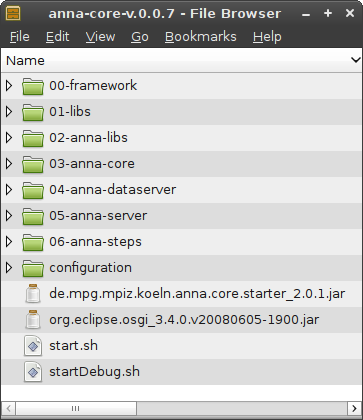
\includegraphics[scale=0.7]{pics/coreDir.png}
	\caption[Verzeichnisstruktur]{
	\textbf{Die Verzeichnisstruktur der Pipeline.}
	}
	\end{center}
	\label{fig:coreDir}
\end{figure}

Das Programm wird über eine batch-Datei gestartet,
die wiederum das OSGi Framework startet:
\begin{verbatim}
start.sh:
java -Xmx1024m -jar org.eclipse.osgi_3.4.0.v20080605-1900.jar
-clean\end{verbatim}
Das OSGi Framework ist so konfiguriert (\code{configuration/config.ini}), dass
es beim Starten automatisch das Bundle
\begin{verbatim}
de.mpg.mpiz.koeln.anna.core.starter_2.0.1.jar
\end{verbatim}
installiert und startet.
Dieses Bundle initialisiert und startet nun die Pipeline, indem es alle Bundles,
die sich in den Verzeichnissen \code{00-} bis \code{06-} befinden,
installiert und startet.
Im Verzeichnis \code{06-} sollten sich dabei alle
Bundles befinden, die Implementierungen von Step bereitstellen und in der
Pipeline genutzt werden sollen.

\section{Implementierungen von Step}
\todo{\dots}

\subsection{Step Commons}

\subsection{Step Commons LSF}

\subsection{InputSequenceReader}

\subsection{Conrad}
Conrad
(\htmladdnormallink{http://www.broadinstitute.org/annotation/conrad/}{http://www.broadinstitute.org/annotation/conrad/})
ist ein \textit{de novo} gene caller, der Genstrukturen wie Exons und Introns
vorhersagen kann.
\index{Conrad} \index{de novo}\index{gene caller}
Die Vorhersage stützt sich dabei auf \textit{semi-Markow Conditional Random
Fields}, kurz \textbf{CRF}.  % wird in hintergründen erwähnt
\index{Markow} \index{Conditional Random Fields} \index{CRF|see{Conditional
Random Fields}}
Conrad benötigt für seine Genvorhersage eine FASTA-Datei mit einer oder
mehreren zu analysierenden DNA-Sequenzen, sowie eine Binärdatei, die Parameter
für den CRF-Alorithmus entält.
Diese Binärdatei wird in einem Trainingslauf erstellt, der vor der
eigentlichen Genvorhersage durchgeführt wird. Hierbei wird der CRF-Algorithmus
auf die Eingabesequenz trainiert, um die Qualität der Genvorhersage
zu maximieren. Dieser Trainingslauf benötigt eine FASTA-Datei mit
DNA-Sequenzen, die Gene enthalten, sowie eine GFF-Datei mit Annotationen zu
diesen Genen.
Die DNA-Sequenzen, die für das Training herangezogen werden, bestimmen direkt
die Qualität der späteren Genvorhersage:
Je \enquote{ähnlicher} die Trainingssequenzen den Sequenzen für die
Vorhersage sind, desto genauer wird das Ergebnis.
\citep{doherty_gene_2007}

Um einen Eindruck von der Qualität der Genvorhersage zu gewinnen, wurden
mehrere Trainings- und Vorhersage-Schritte mit einem Beispieldatensatz aus dem
Conrad-Packet durchgeführt, deren Ergebnisse dann kreuzvalidiert wurden.
Der Beispieldatensatz beinhaltete 574 Sequenzen von \texttt{Aspergillus niger},
die dazu im Verhältnis 1:10 in zwei Datensätze \enquote{testing} und
\enquote{training} aufgeteilt wurden. Das Training erfolgte mit dem
\enquote{training}-Datensatz, die anschliessende Vorhersage wurde für beide
Datensätze durchgeführt.
\index{Aspergillus niger}

Das Ergebnis hieraus war also zum einen eine Vorhersage für eben die Sequenzen,
mit denen Conrad zuvor trainiert wurde, zum Anderen eine Vorhersage für unbekannte
Sequenzen, welcher allerdings ein optimales Training vorrausgegangen war.

Das Ergebnis der Genvorhersage für die beiden Datensätze \enquote{training} und
\enquote{testing} stellt sich wie folgt dar:\\
Die Werte für den \enquote{training}-Datensatz sind generell relativ konstant,
für den \enquote{testing}-Datensatz sind sie weiter gestreut.
Diese Verteilung ist zu erwarten und zeigt ein ausgewogenes Training.
Das bei einem Training oft auftretende \textit{over fitting} ist nicht
festzustellen.
\index{over fitting}
Die Qualität der Genvorhersagen stellt sich in sechs Kategorien dar:
\begin{description}
\item[prediction sensitivity for coding exons] ist das Verhältnis
der gefundenen Exons zu den tatsächlichen vorhandenen Exons.
\item[prediction specificity for coding exons] \ldots
\item[prediction sensitivity for coding nucleotides] \ldots
\item[prediction specificity for coding nucleotides] \ldots
\item[perfectly predicted sequences] ist das Verhältnis aller
vollständig korrekt vorhergesagten Exons zu der Gesamtmenge an Exons.
\item[nucleotide hidden state agreement] ist das Verhältnis der vorhergesagten
Basen-\enquote{Zustände} zu den tatsächlichen Basen-Zuständen.
\end{description}

\begin{figure}[ht]
	\begin{center}
		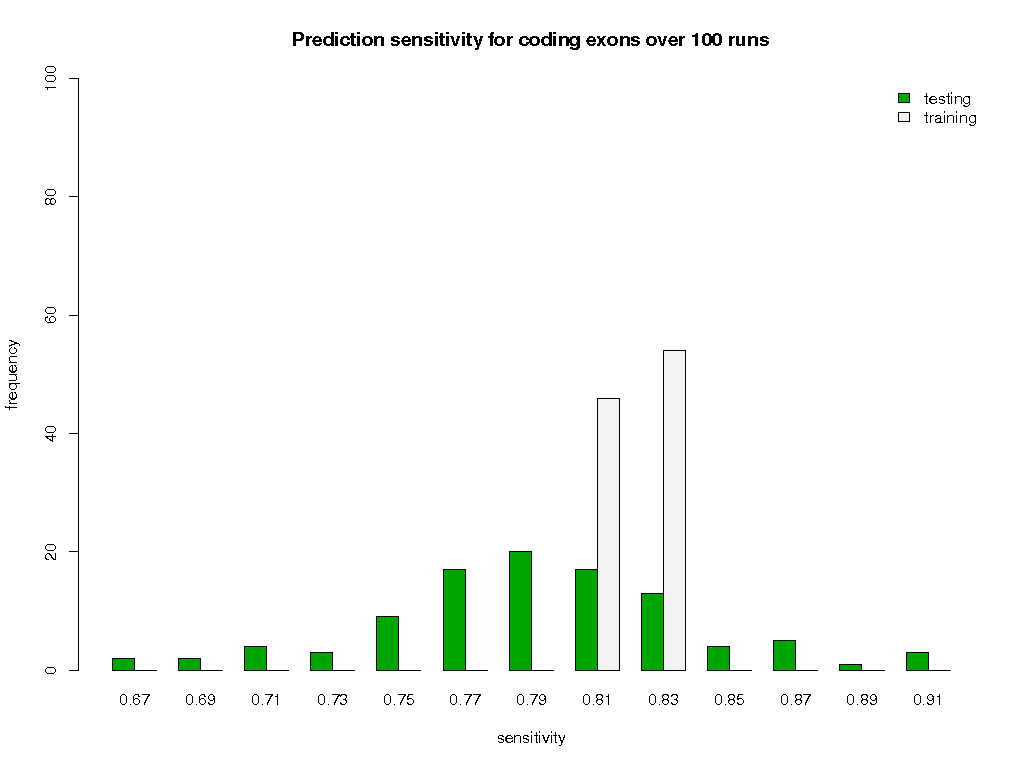
\includegraphics[scale=0.42]{pics/codingExons_sens.png}
	\caption[Prediction sensitivity for coding exons over 100 runs]{
	\textbf{Prediction sensitivity for coding exons over 100 runs.}
	something}
	\end{center}
	\label{fig:codingExons_sens}
\end{figure}

\begin{figure}[ht]
	\begin{center}
		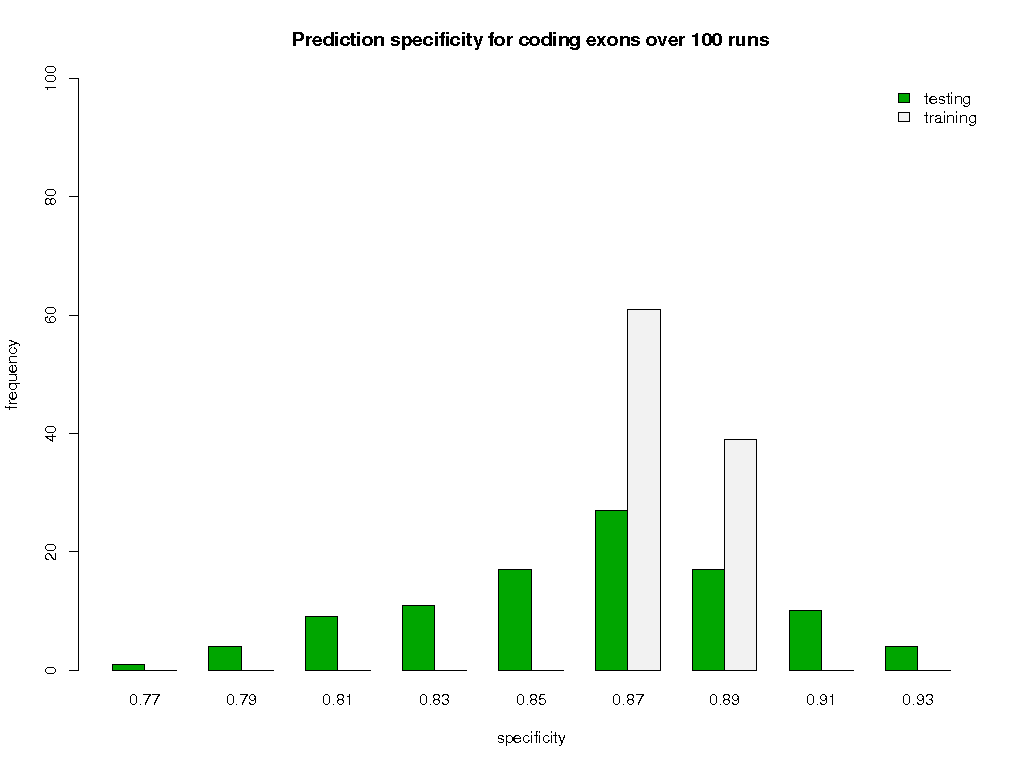
\includegraphics[scale=0.42]{pics/codingExons_spec.png}
	\caption[Prediction specificity for coding exons over 100 runs]{
	\textbf{Prediction specificity for coding exons over 100 runs.}
	something}
	\end{center}
	\label{fig:codingExons_spec}
\end{figure}

\begin{figure}[ht]
	\begin{center}
		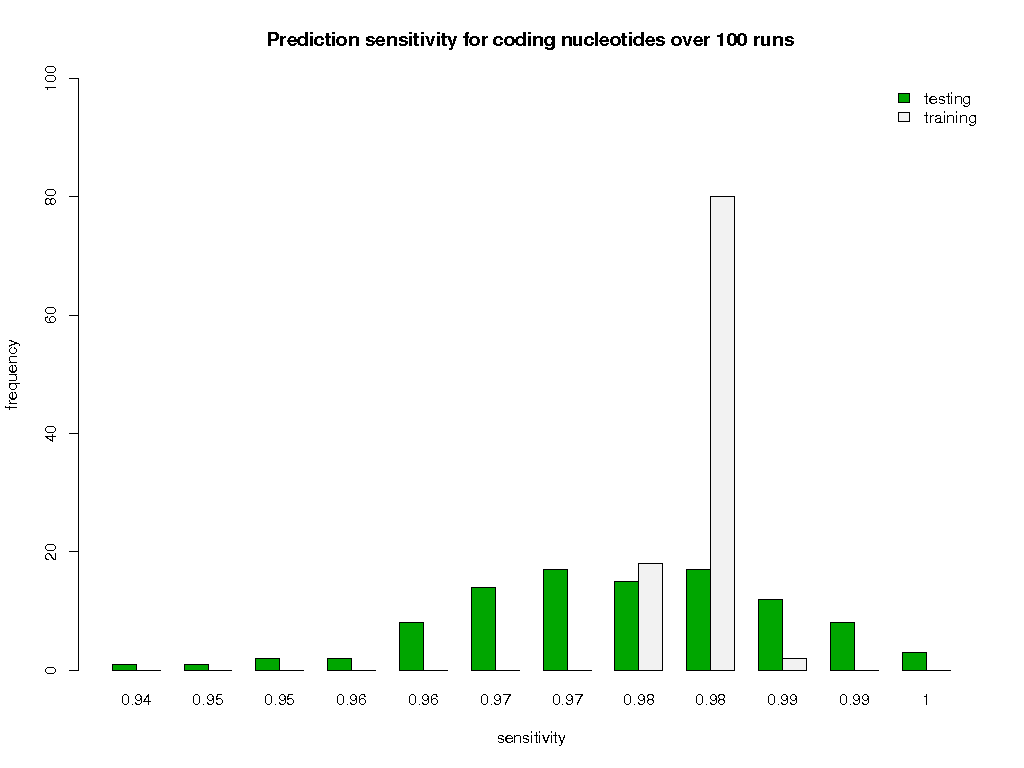
\includegraphics[scale=0.42]{pics/codingNucleotides_sens.png}
	\caption[Prediction sensitivity for coding nucleotides over 100 runs]{
	\textbf{Prediction sensitivity for coding nucleotides over 100 runs.}
	something}
	\end{center}
	\label{fig:codingNucleotides_sens}
\end{figure}

\begin{figure}[ht]
	\begin{center}
		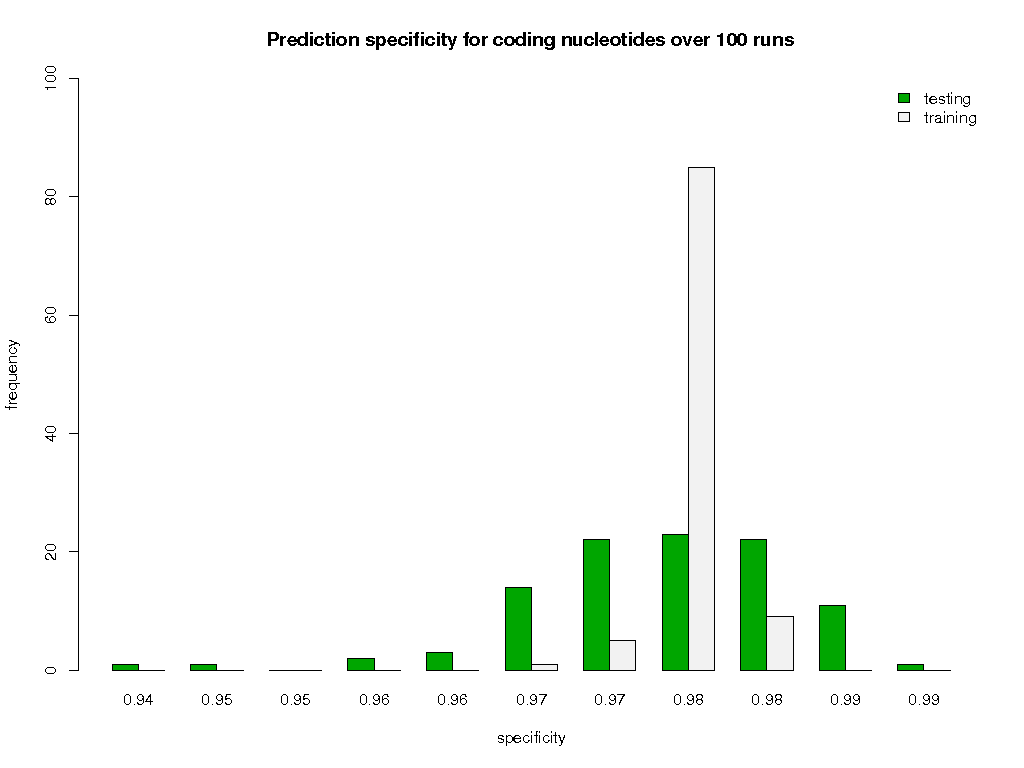
\includegraphics[scale=0.42]{pics/codingNucleotides_spec.png}
	\caption[Prediction specificity for coding nucleotides over 100 runs]{
	\textbf{Prediction specificity for coding nucleotides over 100 runs.}
	something}
	\end{center}
	\label{fig:codingNucleotides_spec}
\end{figure}

\begin{figure}[ht]
	\begin{center}
		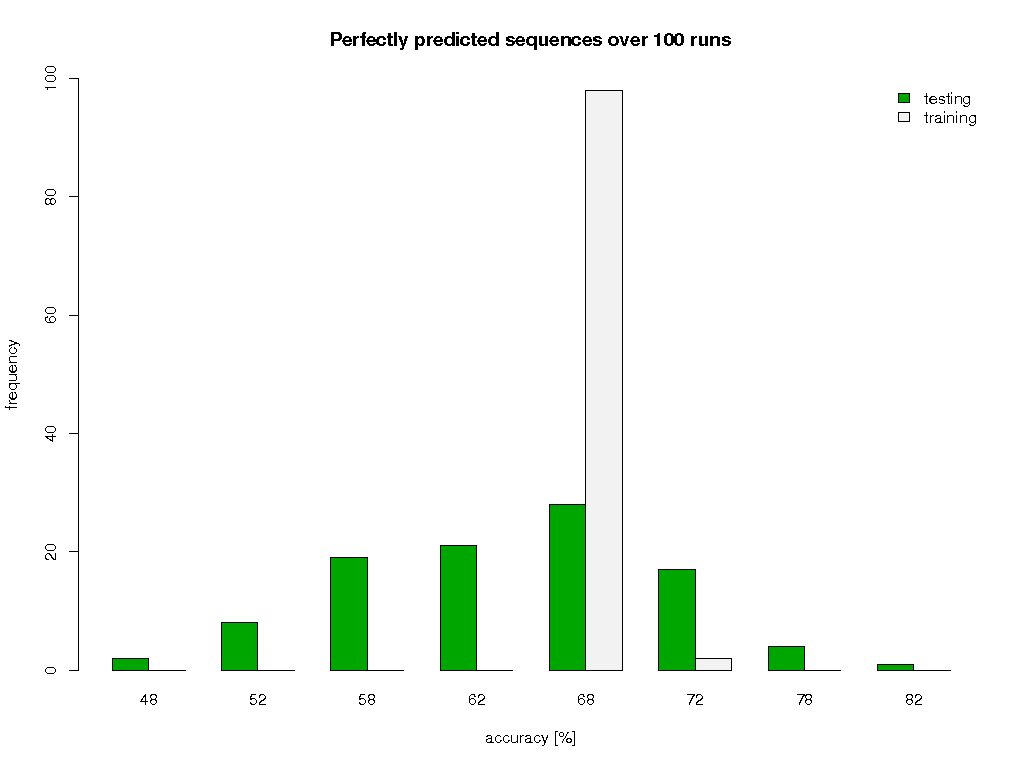
\includegraphics[scale=0.42]{pics/perfect2.png}
	\caption[Perfectly predicted sequences over 100 runs]{
	\textbf{Perfectly predicted sequences over 100 runs.}
	something}
	\end{center}
	\label{fig:perfect2}
\end{figure}

\begin{figure}[ht]
	\begin{center}
		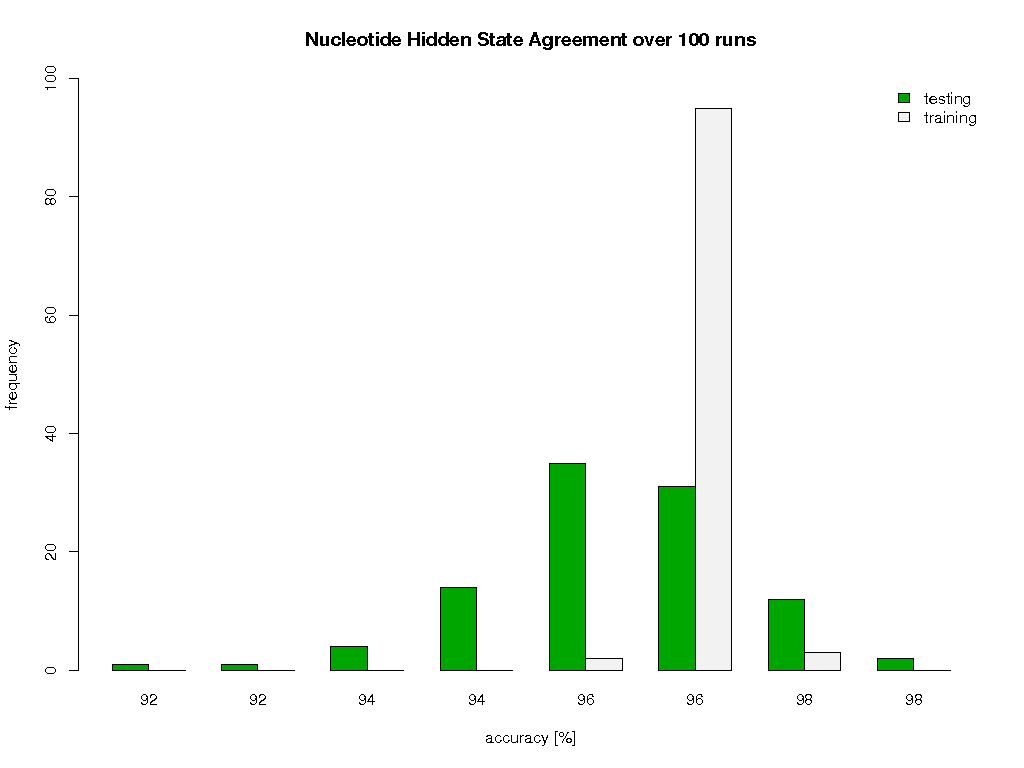
\includegraphics[scale=0.42]{pics/agree2.png}
	\caption[Nucleotide Hidden State Agreement over 100 runs]{
	\textbf{Nucleotide Hidden State Agreement over 100 runs.}
	something}
	\end{center}
	\label{fig:agree2}
\end{figure}

\paragraph{Conrad local}

\paragraph{Conrad LSF}

\paragraph{Get Results}

\subsection{RepeatMasker}
RepeatMasker
(\htmladdnormallink{http://www.repeatmasker.org/}{http://www.repeatmasker.org/})
ist ein Open Source Projekt, das repetetive Elemente einer Sequenz
\enquote{maskiert}, um so Rauschen während ähnlichkeitsbasierter Suchen zu
unterdrücken.
Die Maskierung kann entweder durch das Ersetzten der betroffenen Sequenzen
durch \enquote{N}'s bzw. \enquote{X}'s oder auch durch Ändern der Basen zur
Kleinschreibweise erfolgen.
Letzteres wird beispielsweise von \textit{BLAST} erkannt, was zur Folge hat,
dass diese Sequenzabschnitte nicht in der Suche berücksichtigt werden.
Die ursprüngliche Sequenzinformation bleibt auf diese Weise	erhalten.

\paragraph{RepeatMasker local}

\paragraph{RepeatMasker LSF}

\paragraph{Get Results}

\section{Libraries}
Neben den Basisfunktionalitäten und den bereits erwähnten Steps
beinhaltet Anna noch verschiedene Bundles, die Klassen aus externen Libraries
bereitstellen:
\begin{description}
\item[bioutils] dieses Bundle enthält eine Sammlung
von Klassen, die speziell bioinformatische Funktionalitäten bereitstellen.
\todo{gogo, johnny go}
\item[kerner.commons] stellt die Klassen aus dem Paket
\name{kerner-commons} bereit. basic java functionallity, like convenient IO or
String operations
\end{description}
